\section{Other Optimisations and Parallelism}

In this section general optimisations used throughout the algorithm will be described.
These were not discussed during the general discussion of the two phases as they were not necessary to understand those topics, and they would have added a lot of complexity to an already complex topic.

\subsection{Curiously Recurring Template Pattern (CRTP)}

The first and simplest optimisation is the Curiously Recurring Template pattern which is popular for C++ development.
For those unfamiliar with C++, when a child class inherits a parent class and polymorphism takes place, a virtual table is created, which indicates the correct function to call to the program.
Thus, when a call to an inherited function is done, another call to the virtual table must be done, which is usually expensive as it requires another memory access.
CRTP allows programmers to do inheritance without the need for virtual tables, with the penalty being the use of templates, which make the code slightly less maintainable.
This optimisation was especially beneficial for the results printing, as some of the methods there are called billions of times, and traditional inheritance is still used in a lot of places where methods are not called as often.

\subsection{Multithreaded Pipeline}

In the two phases, there are some components that are dependent on one another, and others that are not.
Furthermore, since it is a pipeline, an earlier component can start processing the next batch while the later component is processing an earlier batch.
This is done by inheriting all producer components from a parent component called the \textit{SharedBatchesProducer}.
By using semaphores, it is ensured that all components can run in parallel, while still being able to share the memory of the buffers that the producers and consumers share safely.

\subsection{Pinned Memory}

For variables that need to be copied to and from the GPU, it is possible to use pinned memory on the main memory in order to speed up memory transfers.
To do this, all the programmer needs to do is to reserve the memory space beforehand using \textit{cudaMallocHost}\footnote{\url{https://docs.nvidia.com/cuda/cuda-runtime-api/group__CUDART__MEMORY.html}} or \textit{hipHostMalloc}\footnote{\url{https://rocm-developer-tools.github.io/HIP/group__Memory.html}} if using HIP.
Pinned memory can be copied to the GPU directly, whereas more care needs to be taken by pageable memory as this could be moved while copying is taking place, whereas pinned memory is guaranteed to remain in the same location within memory until it is freed\footnote{\url{https://developer.nvidia.com/blog/how-optimize-data-transfers-cuda-cc/}}.
This feature sped up transfers to and from GPU by almost twice, which is a significant difference for this use case as there are a lot of large transfers.
The drawback of reserving most of the memory beforehand is that large amounts of contiguous blocks need to be reserved at once.
This can be difficult to manage for the operating system, and in fact often contributes to a significant overhead at the start of the algorithm
Luckily this overhead is constant, so as the datasets get larger, this overhead becomes less and less significant, and for smaller datasets, a smaller memory can be reserved for the algorithm, which is a setting that can be altered by the user.
That said, for other variables which do not need to be communicated to or from the GPU, normal paged memory is used.

\subsection{Streams}

Often, larger datasets will be split into multiple files.
The code takes advantage of this by providing an algorithm that can take advantage of this, by being able to process multiple files at once.
This means that the pipeline is duplicated and the number of files can be split between each stream.
The term \textit{stream} is used to indicate each pipeline.
This means that, for example, given seven files and three streams, then stream 0 would handle three files, and streams 1 and 2 would handle two files each.
The two streams can then share the same SBWT or colors data structure in phases 1 and 2 respectively.

The benefit of using streams is that reading from disk and outputting to disk can also be done in parallel.
This is especially useful when using a multi-disk setup, or if the device in use can support this feature.
However, even if not using any of the above two hardware devices, two more advantages are universally applicable.
The first and more obvious is that by using streams, the CPU and disk can be kept more busy.
The second is the use of GPU streams.

Using a single stream with GPUs, the process is: (a) copy some data to the GPU, (b) do some processing, and (c) copy the data back to main memory.
By using multiple streams, each stream still does the same three steps, however, if multiple streams are used, the GPU can interleave the memory transfer of one stream with the processing of another\footnote{\url{https://developer.download.nvidia.com/CUDA/training/StreamsAndConcurrencyWebinar.pdf}}.
Memory transfers from GPU can also be interleaved with memory transfers to GPU on some devices.
Figure~\ref{fig:Streams} shows this visually.
The number of streams is configurable by the user, but is capped based on the number of files, so that the number of streams is always smaller or equal to the number of files that need to be processed.

\begin{figure}[t]
  \centering
  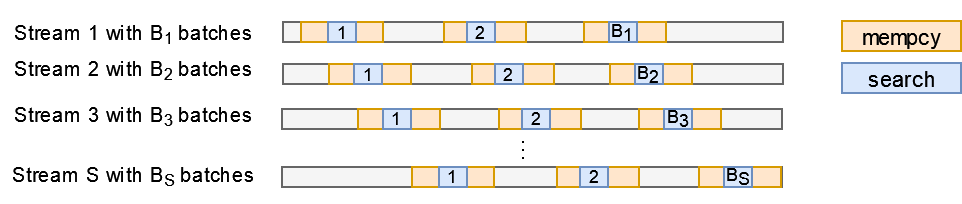
\includegraphics[width=0.8\textwidth]{images/Streams.png}
  \caption{A visualisation of using streams and their benefit on GPU processing, where memory transfers are interleaved with processing. The batch number is also displayed.}\label{fig:Streams}
\end{figure}

\subsubsection{Load Balancing}

An additional optimisation for streams is to load balance the streams.
Notice that if some files are large while others are very small, then different streams might have very different workloads.
Thus, the algorithm considers load to be based on file size.
As such, before assigning files to streams, they are analysed for their size and then a greedy algorithm called the Longest Processing Time first (LPT)~\cite{LPT1, LPT2}.
Here, an array is created for each stream, the file sizes are sorted such that the largest file is always chosen first and this file is then assigned to the array with the smallest load.
LPT is proven to be bound to give a result that is $\frac{4}{3}$ from the optimal~\cite{LPT2}.
This load balancing is done in both phases.

\subsection{Memory Reservations}

When it comes to memory reservations, all the memory allowed by the user through user input is reserved by the algorithm.
This first checks how much memory each component needs per character or per index, in phases 1 and 2 respectively, and then reserves memory accordingly, such that the batches are as big as possible without overflowing GPU or main memory.
When the algorithm has multiple streams, this memory reserved is divided by the number of streams, such that each stream gets an equal amount of memory, and thus the batch sizes are equal.
Figures~\ref{fig:IndexBatches} and~\ref{fig:ColorBatches} in Appendix~\ref{app:Batches} shows all the dependent components and the memory needed by each component.
